%% Requires compilation with XeLaTeX or LuaLaTeX.
\documentclass[10pt,xcolor={table,dvipsnames},t]{beamer}
\usetheme{UCBerkeley}

\usepackage{amsmath}
\usepackage{booktabs}
\usepackage{graphicx}
\usepackage{tikz}
\usetikzlibrary{positioning,arrows.meta}

\graphicspath{
  {../result/summary_plots/}
  {../result/eda/}
  {../result/gradcam/resnet18_unfrozen_from_frozen_lr1e-4_128_e8/gradcam_20260508_104648/}
}

\title[Food Image Classification]{Transfer Learning for Binary Food Image Classification}
\subtitle{INDENG 1/242B Spring 2026 Project}
\author{Xutong Dong \and Zhaoning Liang \and Yirong Li \and Jiaxu Zhang}
\institute{University of California, Berkeley}
\date{May 2026}

\setbeamerfont{title}{family=\rmfamily,size=\LARGE}
\setbeamerfont{author}{size=\normalsize}

\newcommand{\healthy}{healthy}
\newcommand{\unhealthy}{unhealthy}
\newcommand{\best}[1]{\textbf{\color{Medalist}#1}}

\begin{document}

% Slide 1
\begin{frame}
  \titlepage
\end{frame}

\smallframetitle

% Slide 2
\begin{frame}{Motivation and Learning Problem}
\footnotesize
\begin{columns}[T]
\begin{column}{0.52\textwidth}
\begin{block}{Use case}
Coarse food-image screening: classify a food image as \healthy{} or \unhealthy{}.
\end{block}
\begin{itemize}
  \item Input feature: RGB food image \(x\).
  \item Label: \(y\in\{\healthy,\unhealthy\}\).
  \item Learned mapping: \(f_\theta(x)\rightarrow y\).
  \item Goal: compare a task-specific CNN with transfer learning and fine-tuning.
\end{itemize}
\end{column}
\begin{column}{0.43\textwidth}
\begin{block}{Project questions}
\begin{itemize}
  \item How strong is a small CNN baseline?
  \item How much does ImageNet transfer help?
  \item Does fine-tuning improve the transferred model?
  \item What errors remain?
\end{itemize}
\end{block}
\end{column}
\end{columns}
\end{frame}

% Slide 3
\begin{frame}{Dataset and Preprocessing}
\footnotesize
\begin{columns}[T]
\begin{column}{0.42\textwidth}
\begin{table}
\centering
\begin{tabular}{lrrr}
\tableheadrow
\tableheadcol{Split} & \tableheadcol{H} & \tableheadcol{U} & \tableheadcol{Total} \\
Train & 2089 & 2089 & 4178 \\
Val. & 261 & 261 & 522 \\
Test & 261 & 261 & 522 \\
\end{tabular}
\end{table}
\begin{itemize}
  \item 5,222 total images.
  \item Balanced classes in every split.
  \item Images resized to \(128\times128\).
  \item Training: crop, flip, color jitter.
  \item Evaluation: resize, center crop, ImageNet normalization.
\end{itemize}
\end{column}
\begin{column}{0.54\textwidth}
\includegraphics[width=\textwidth,height=0.25\textheight,keepaspectratio]{dataset_counts.png}
\vspace{0.2em}
\includegraphics[width=\textwidth,height=0.26\textheight,keepaspectratio]{sample_grid_train.png}
\end{column}
\end{columns}
\end{frame}

% Slide 4
\begin{frame}{Methodology}
\footnotesize
\begin{columns}[T]
\begin{column}{0.48\textwidth}
\begin{block}{Models}
\begin{itemize}
  \item Simple CNN: Conv--BatchNorm--ReLU blocks, max pooling, adaptive average pooling, dropout, linear head.
  \item Frozen ResNet18: ImageNet encoder fixed, binary head trained.
  \item Fine-tuned ResNet18: layer4-only and full-backbone variants.
  \item Advanced extension: supervised contrastive pretraining.
\end{itemize}
\end{block}
\end{column}
\begin{column}{0.48\textwidth}
Classifier probabilities:
\[
 p_\theta(y=c\mid x)=
 \frac{\exp z_c}{\sum_{k=1}^{2}\exp z_k}.
\]
Regularized objective:
\[
 \min_\theta
 \frac{1}{N}\sum_{i=1}^{N}
 L_{\mathrm{ce}}\!\left(f_\theta(x_i),y_i\right)
 +\lambda\lVert\theta_{\mathrm{train}}\rVert_2^2.
\]
\begin{itemize}
  \item Optimizer: AdamW.
  \item Regularization: weight decay, dropout, augmentation, early stopping.
\end{itemize}
\end{column}
\end{columns}
\end{frame}

% Slide 5
\begin{frame}{Experimental Pipeline}
\scriptsize
\begin{center}
\begin{tikzpicture}[
  node distance=0.38cm,
  stage/.style={draw=BerkeleyBlue, rounded corners=2pt, align=center, minimum width=0.82\textwidth, minimum height=0.39cm, fill=BerkeleyTableBlue2},
  arrow/.style={-{Latex[length=2mm]}, thick, BerkeleyBlue}
]
\node[stage] (eda) {EDA and balanced train/validation/test split};
\node[stage, below=of eda] (base) {Simple CNN baseline};
\node[stage, below=of base] (transfer) {Frozen ImageNet-pretrained ResNet18};
\node[stage, below=of transfer] (fine) {ResNet18 partial and full fine-tuning ablation};
\node[stage, below=of fine] (supcon) {Supervised contrastive branch for representation learning};
\node[stage, below=of supcon] (eval) {Held-out metrics, curves, confusion matrices, Grad-CAM, error analysis};
\draw[arrow] (eda) -- (base);
\draw[arrow] (base) -- (transfer);
\draw[arrow] (transfer) -- (fine);
\draw[arrow] (fine) -- (supcon);
\draw[arrow] (supcon) -- (eval);
\end{tikzpicture}
\end{center}
\vspace{0.1em}
The pipeline covers problem formulation, network design, objective, optimizer, regularization, advanced method, and evaluation diagnostics.
\end{frame}

% Slide 6
\begin{frame}{Training and Validation Diagnostics}
\footnotesize
\begin{columns}[T]
\begin{column}{0.5\textwidth}
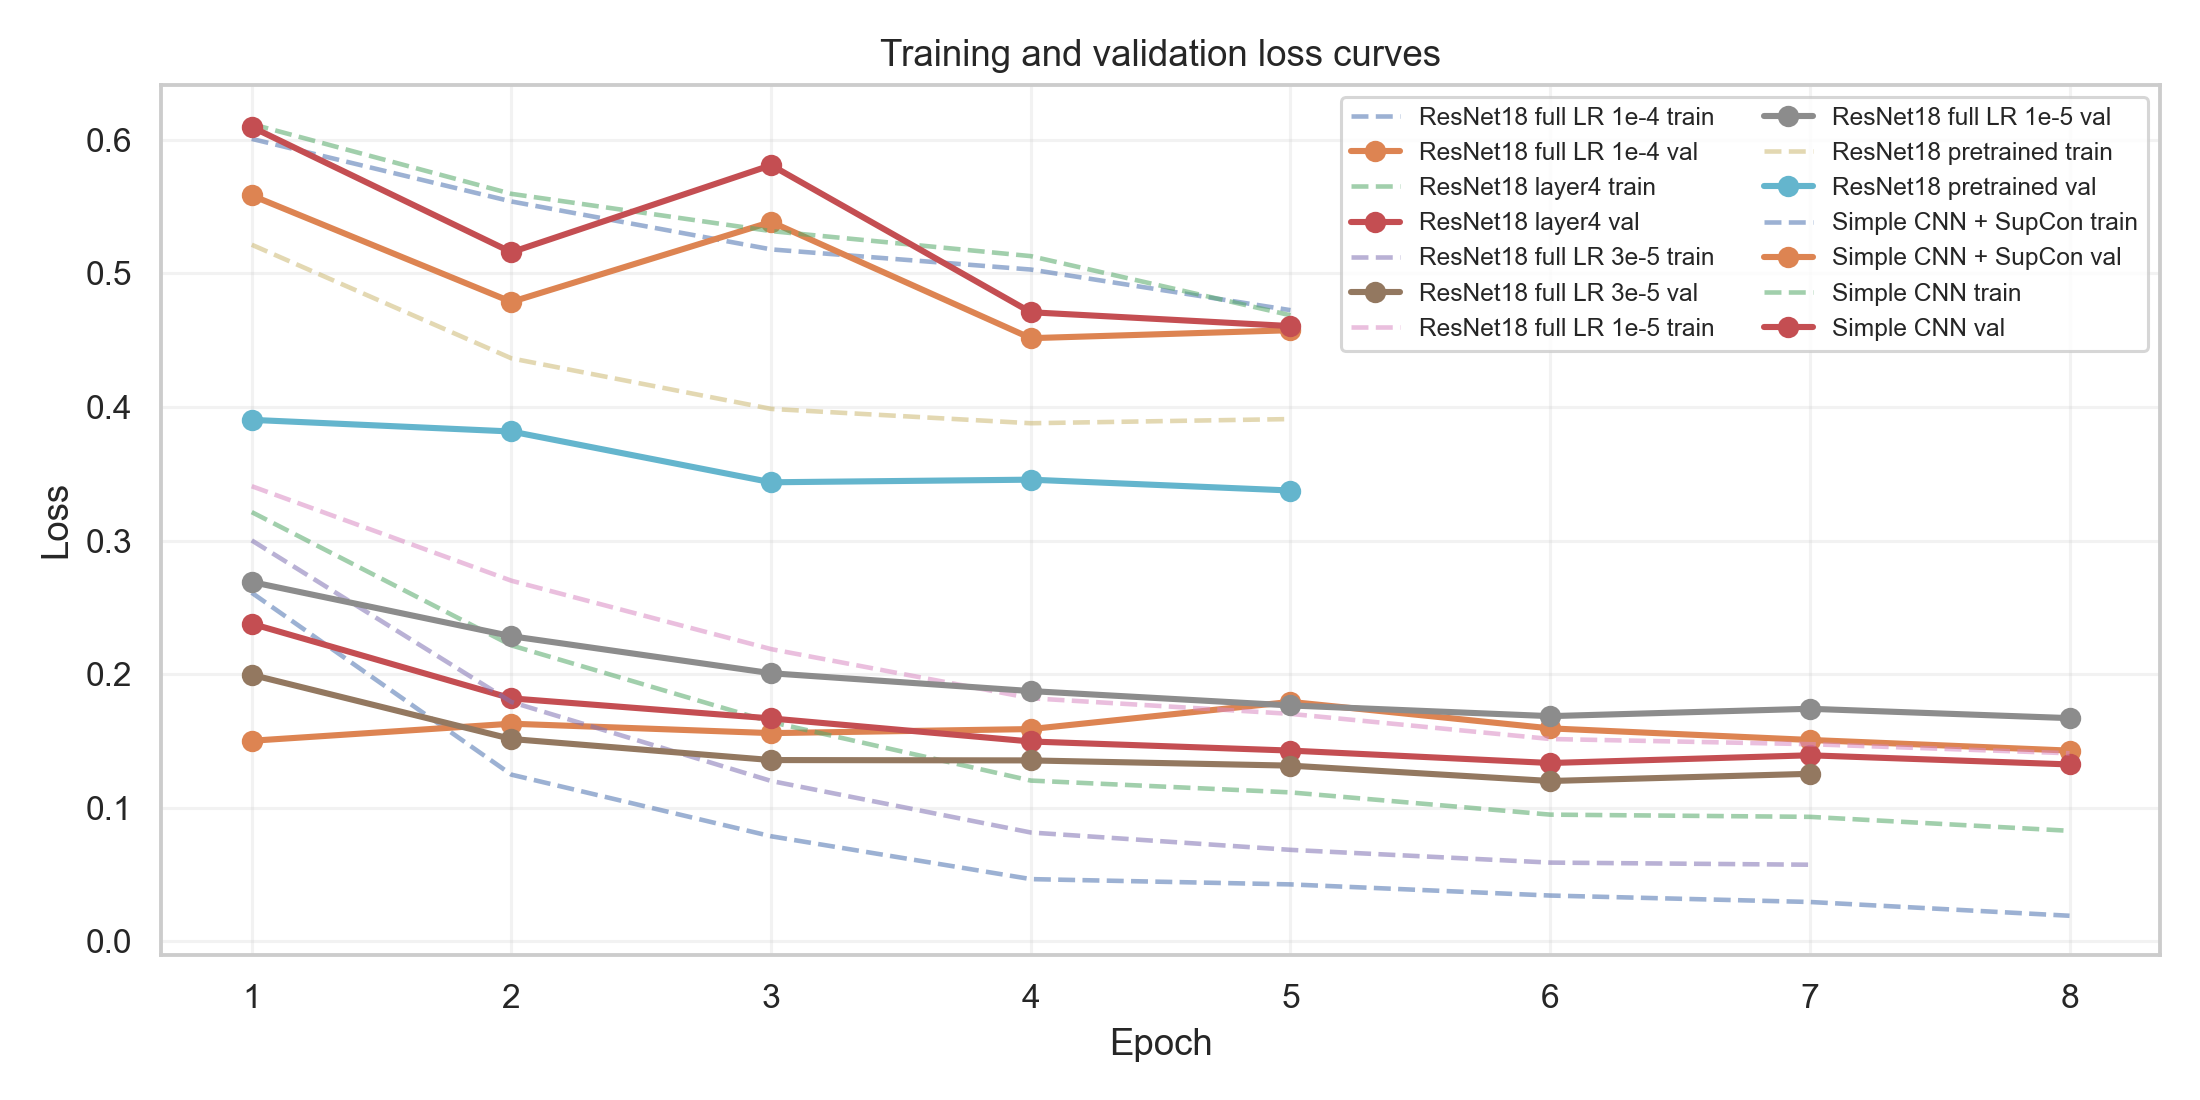
\includegraphics[width=\textwidth,height=0.52\textheight,keepaspectratio]{training_loss_curves.png}
\end{column}
\begin{column}{0.5\textwidth}
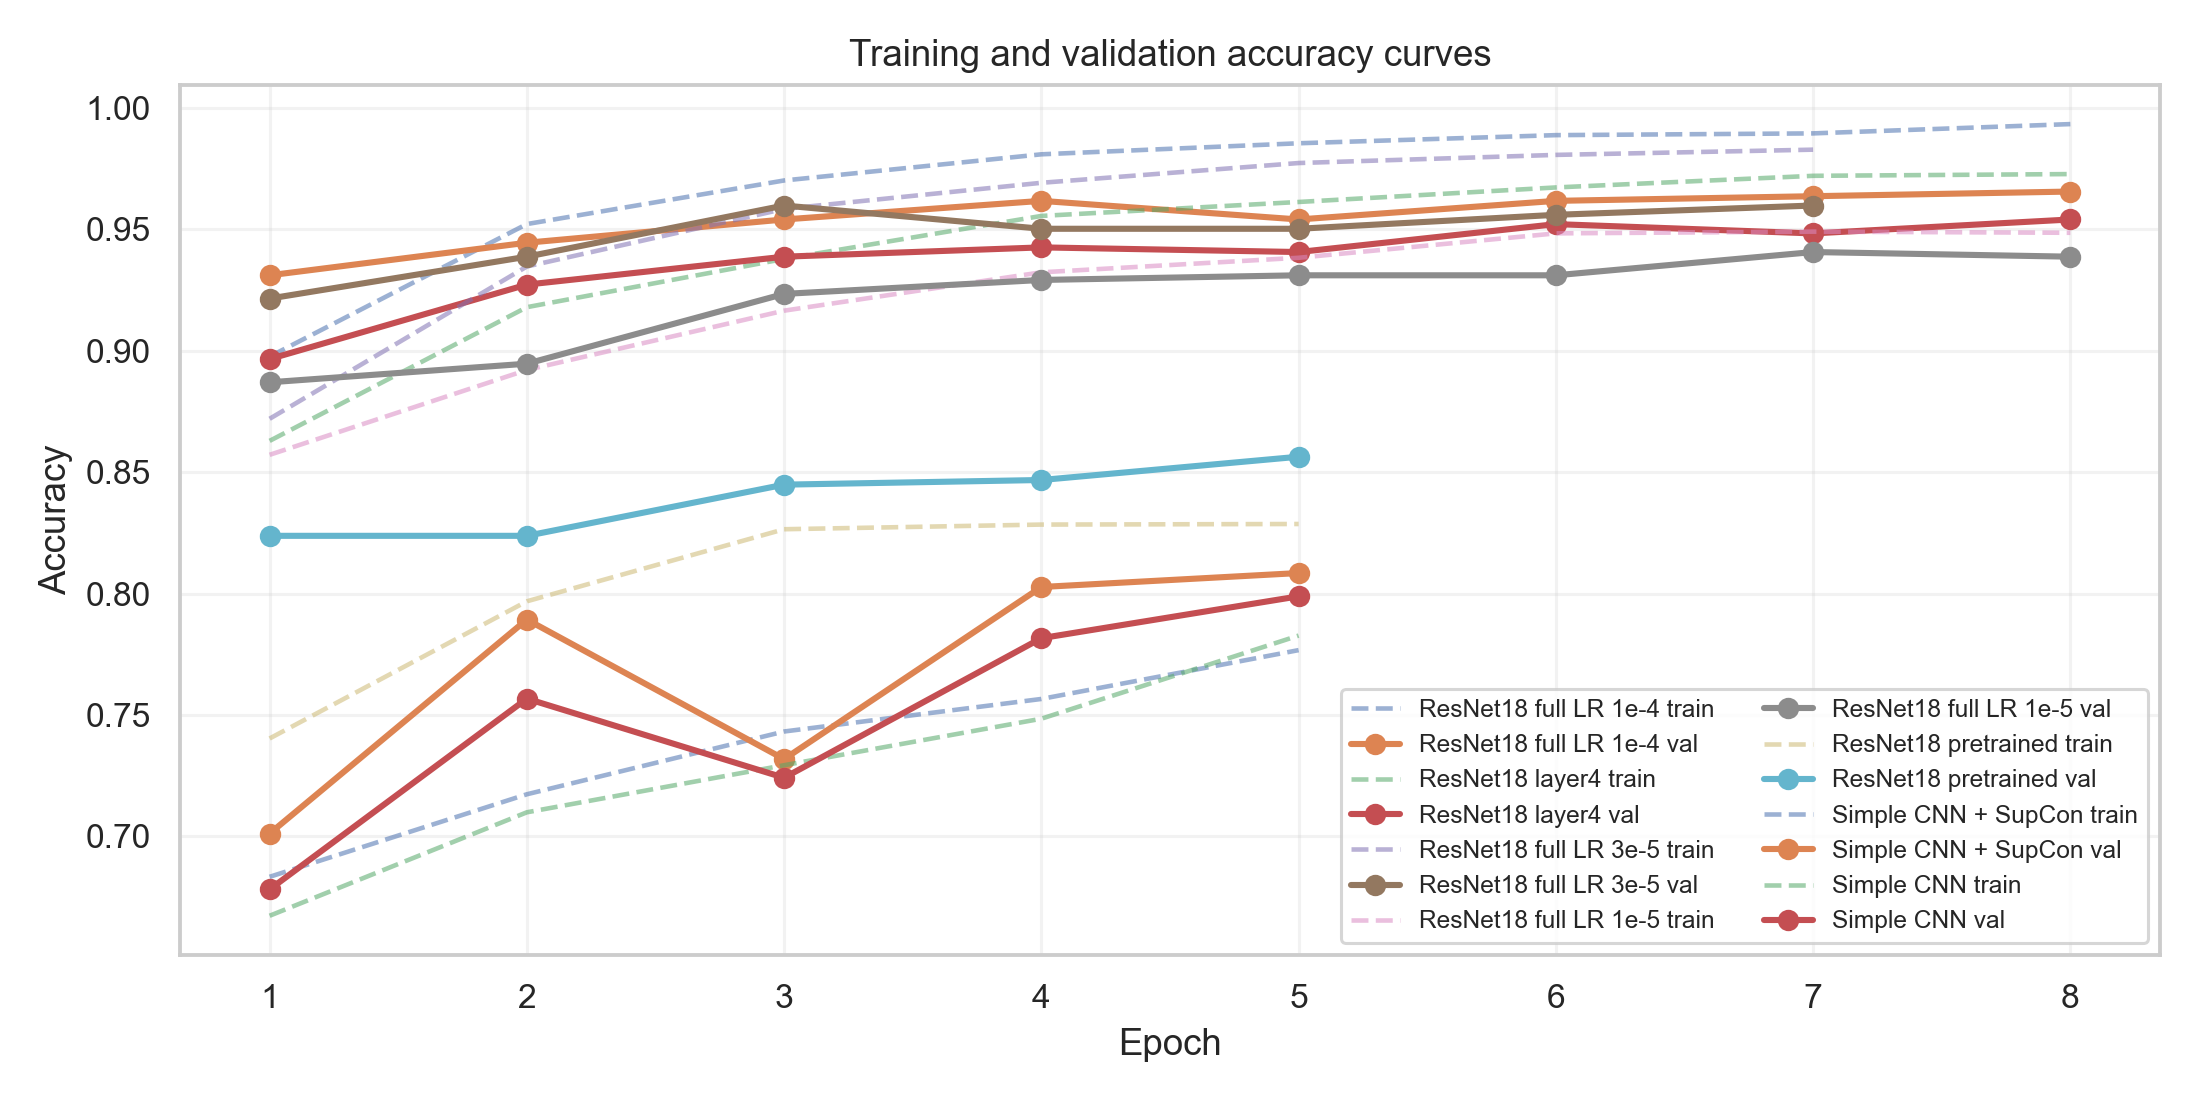
\includegraphics[width=\textwidth,height=0.52\textheight,keepaspectratio]{training_accuracy_curves.png}
\end{column}
\end{columns}
\vspace{0.3em}
\begin{itemize}
  \item Simple CNN variants underfit relative to the transferred ResNet18 family.
  \item Best fine-tuned ResNet18 keeps improving validation accuracy through the final epoch.
  \item A larger train--validation gap appears during fine-tuning, so validation monitoring is necessary.
\end{itemize}
\end{frame}

% Slide 7
\begin{frame}{Main Results}
\scriptsize
\begin{table}
\centering
\begin{tabular}{lrrrr}
\tableheadrow
\tableheadcol{Experiment} & \tableheadcol{Val.} & \tableheadcol{Test} & \tableheadcol{F1} & \tableheadcol{AUC} \\
ResNet18 full fine-tune, LR \(10^{-4}\) & \best{0.9655} & \best{0.9617} & \best{0.9617} & \best{0.9944} \\
ResNet18 layer4 fine-tune, LR \(3{\times}10^{-5}\) & 0.9540 & 0.9406 & 0.9406 & 0.9850 \\
ResNet18 full fine-tune, LR \(3{\times}10^{-5}\) & 0.9598 & 0.9406 & 0.9406 & 0.9845 \\
ResNet18 frozen backbone & 0.8563 & 0.8697 & 0.8697 & 0.9344 \\
Simple CNN + SupCon fine-tune & 0.8084 & 0.8046 & 0.8033 & 0.8813 \\
Simple CNN baseline & 0.7989 & 0.8027 & 0.8027 & 0.8869 \\
\end{tabular}
\end{table}
\vspace{0.3em}
\begin{columns}[T]
\begin{column}{0.52\textwidth}
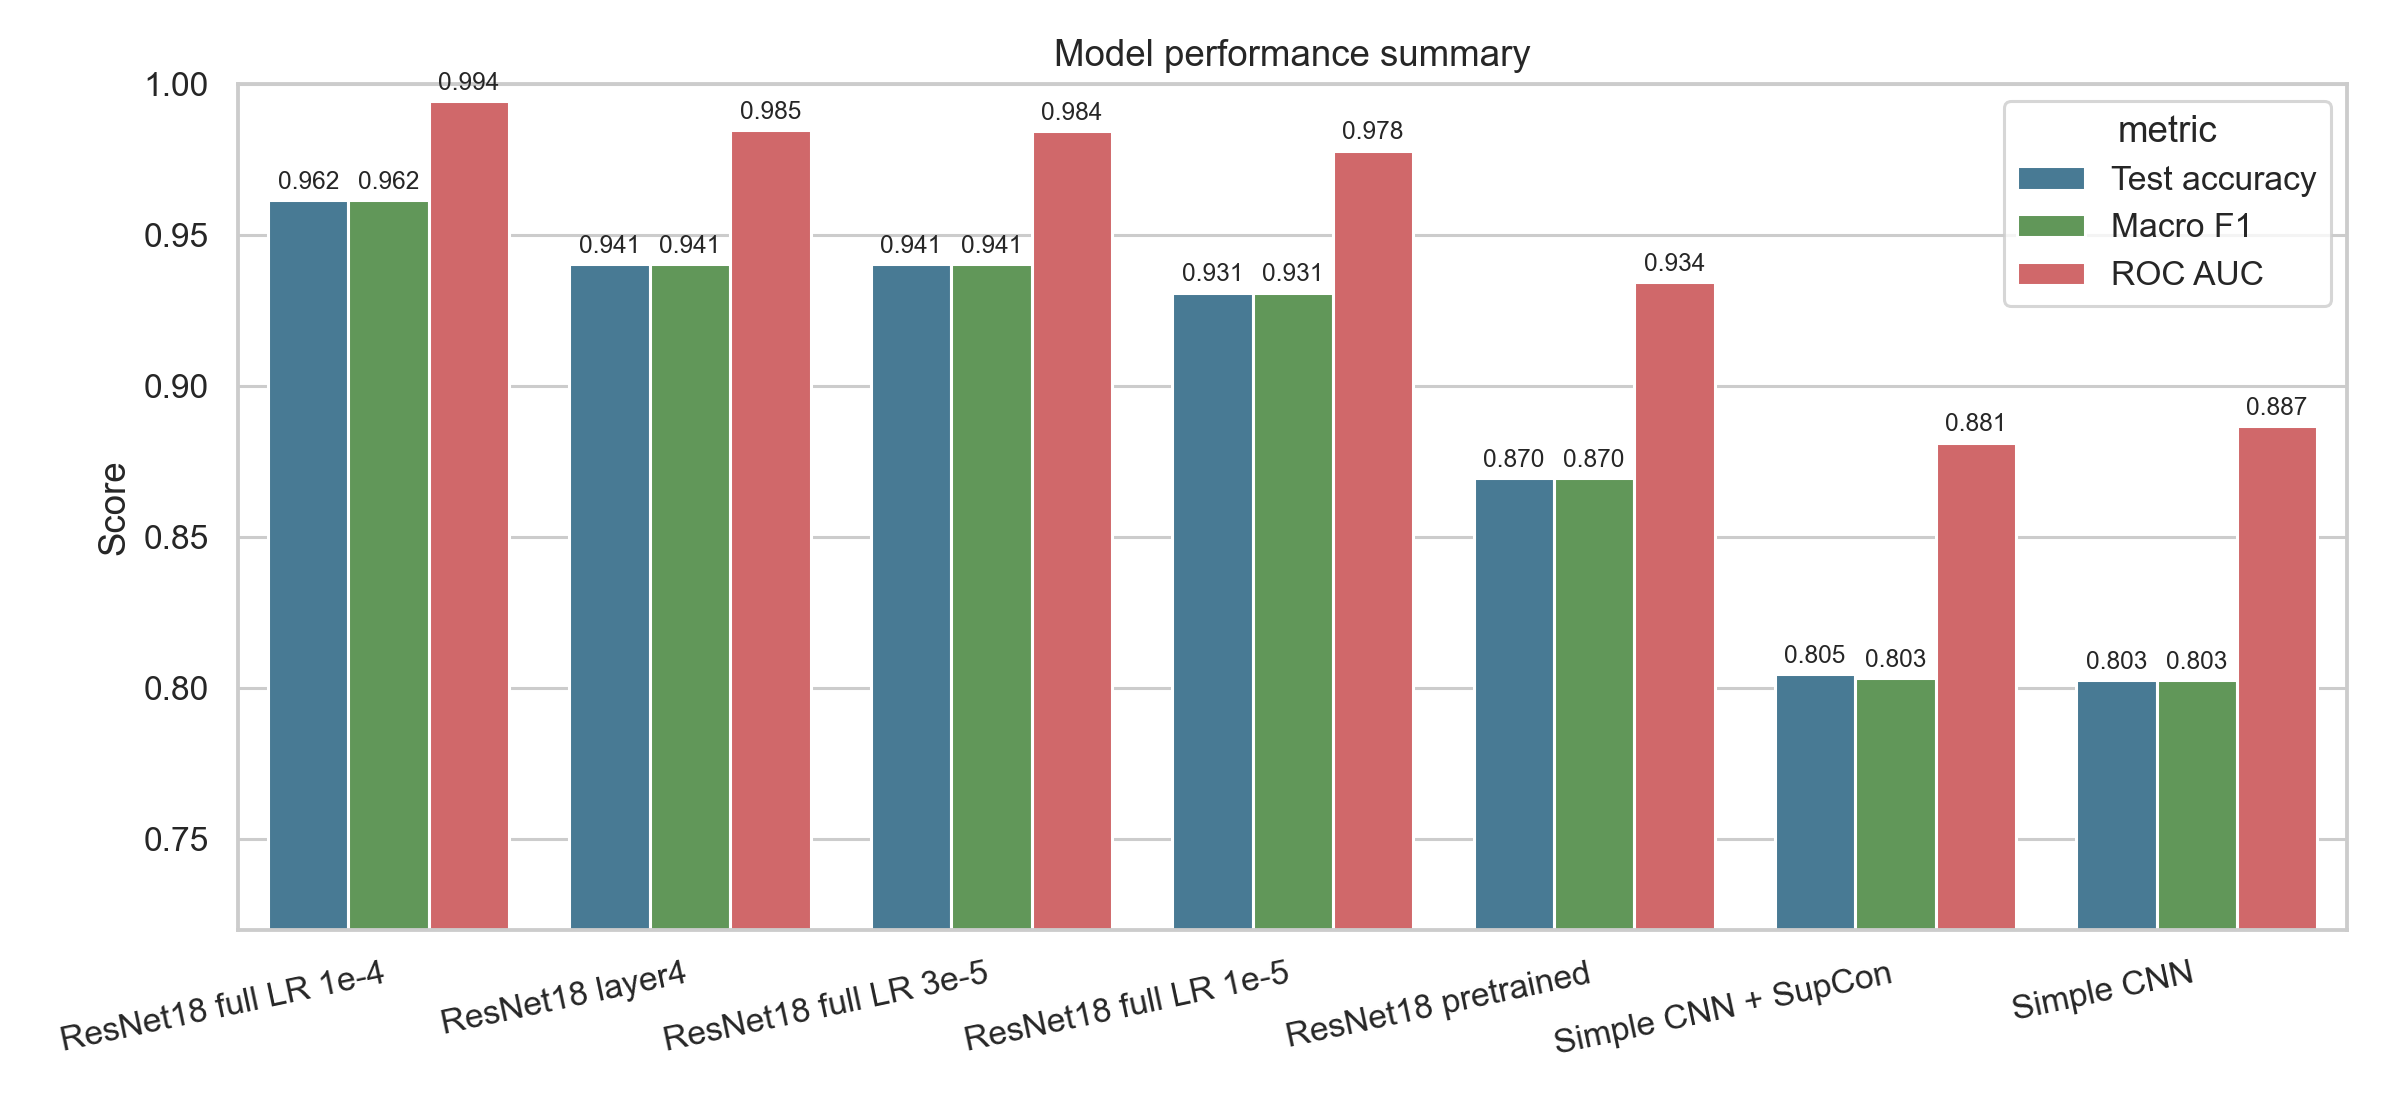
\includegraphics[width=\textwidth,height=0.25\textheight,keepaspectratio]{model_metric_comparison.png}
\end{column}
\begin{column}{0.43\textwidth}
\footnotesize
\begin{block}{Practical improvement}
Full fine-tuning improves test accuracy from \(0.8697\) to \(0.9617\): a \(9.20\)-point absolute gain over frozen transfer.
\end{block}
\end{column}
\end{columns}
\end{frame}

% Slide 8
\begin{frame}{Ablation and Error Analysis}
\footnotesize
\begin{columns}[T]
\begin{column}{0.48\textwidth}
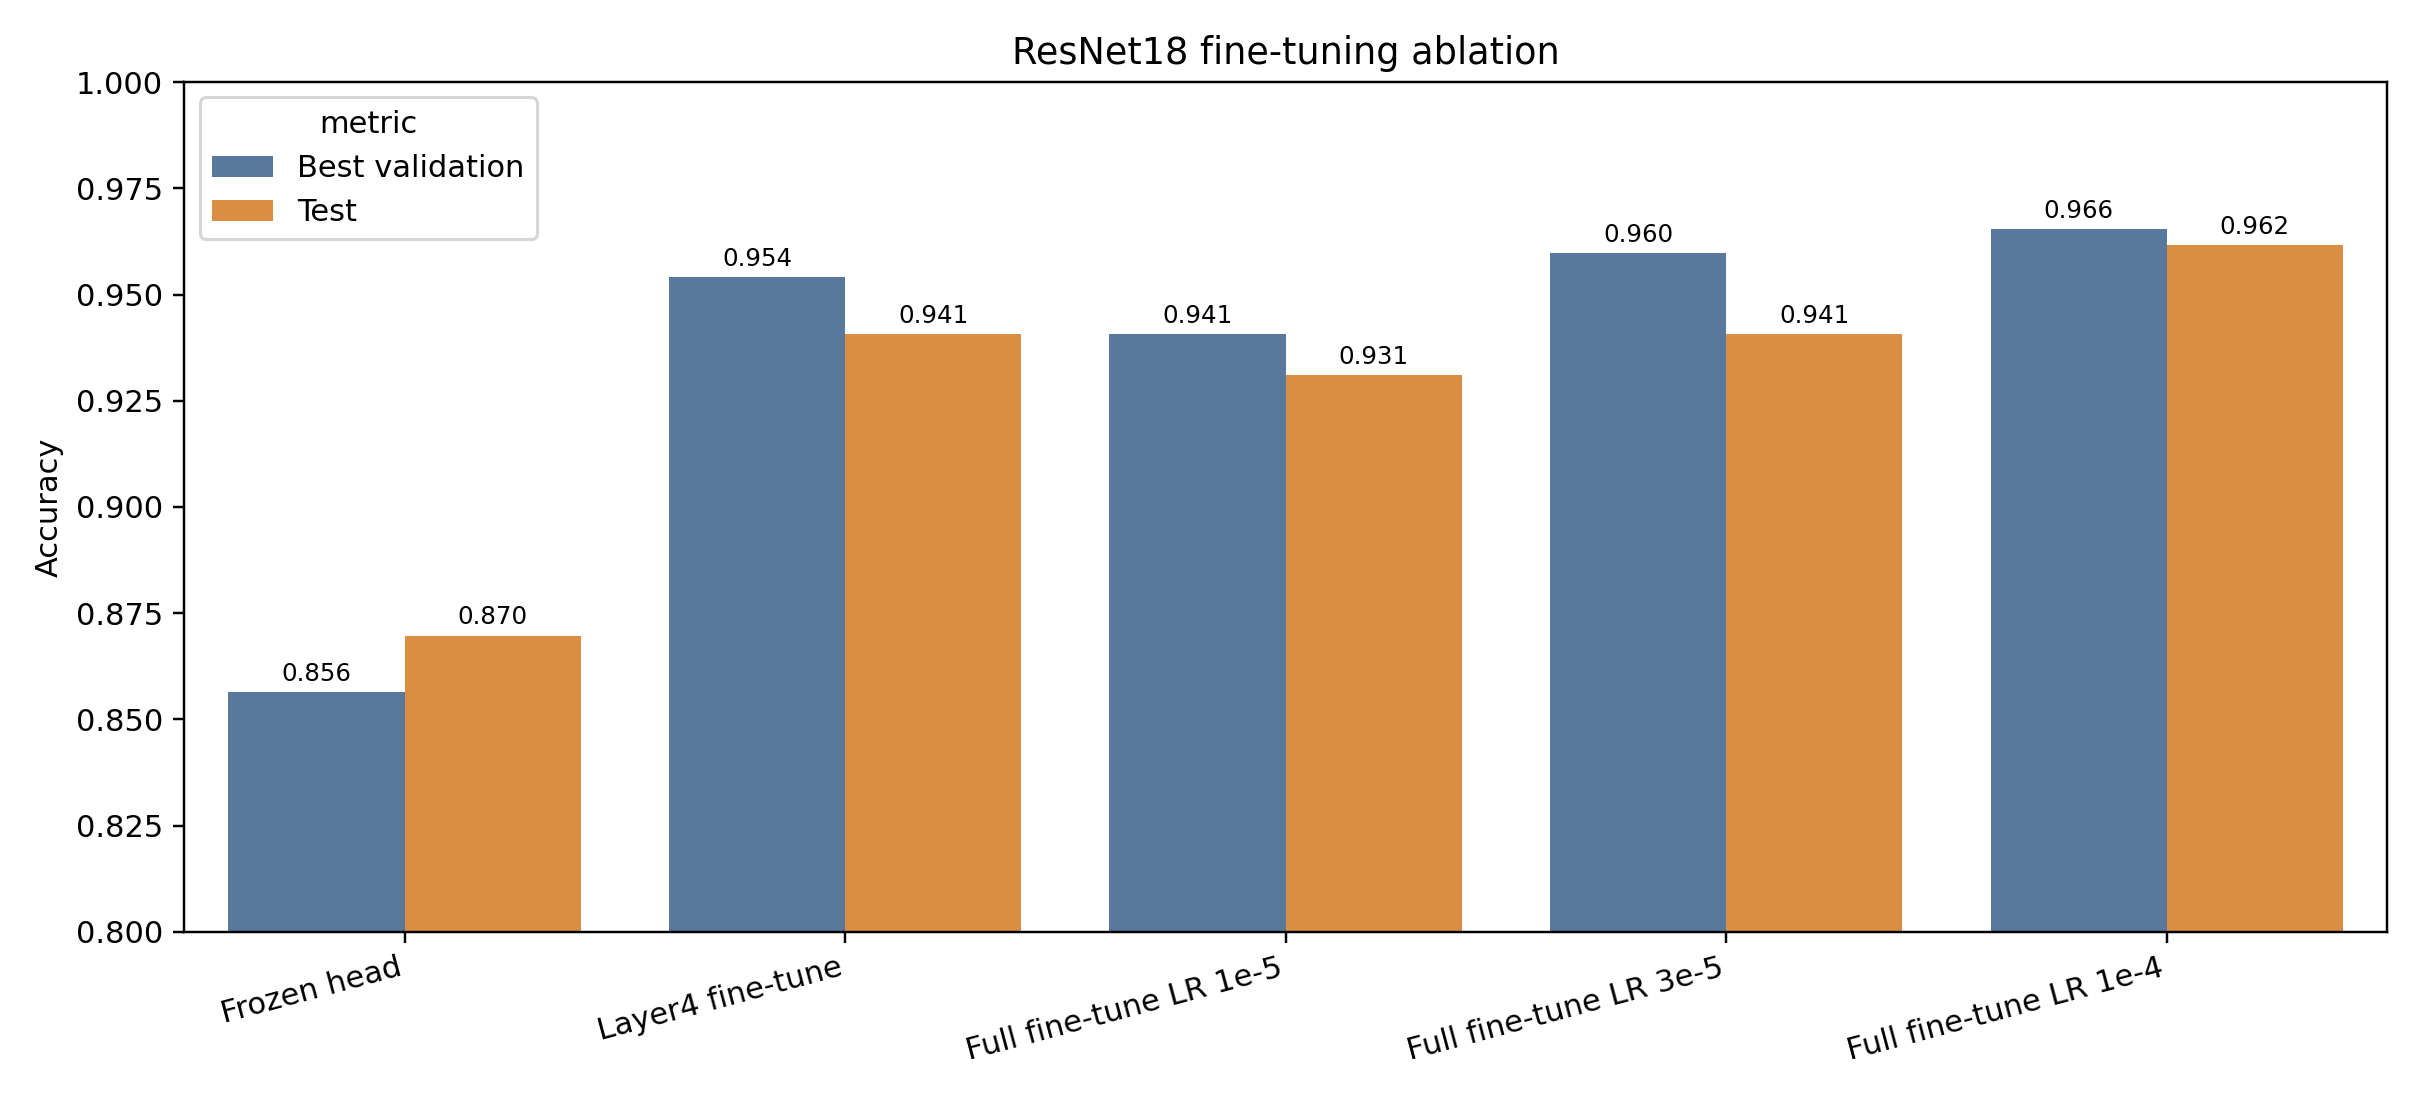
\includegraphics[width=\textwidth,height=0.25\textheight,keepaspectratio]{resnet18_ablation_accuracy.png}
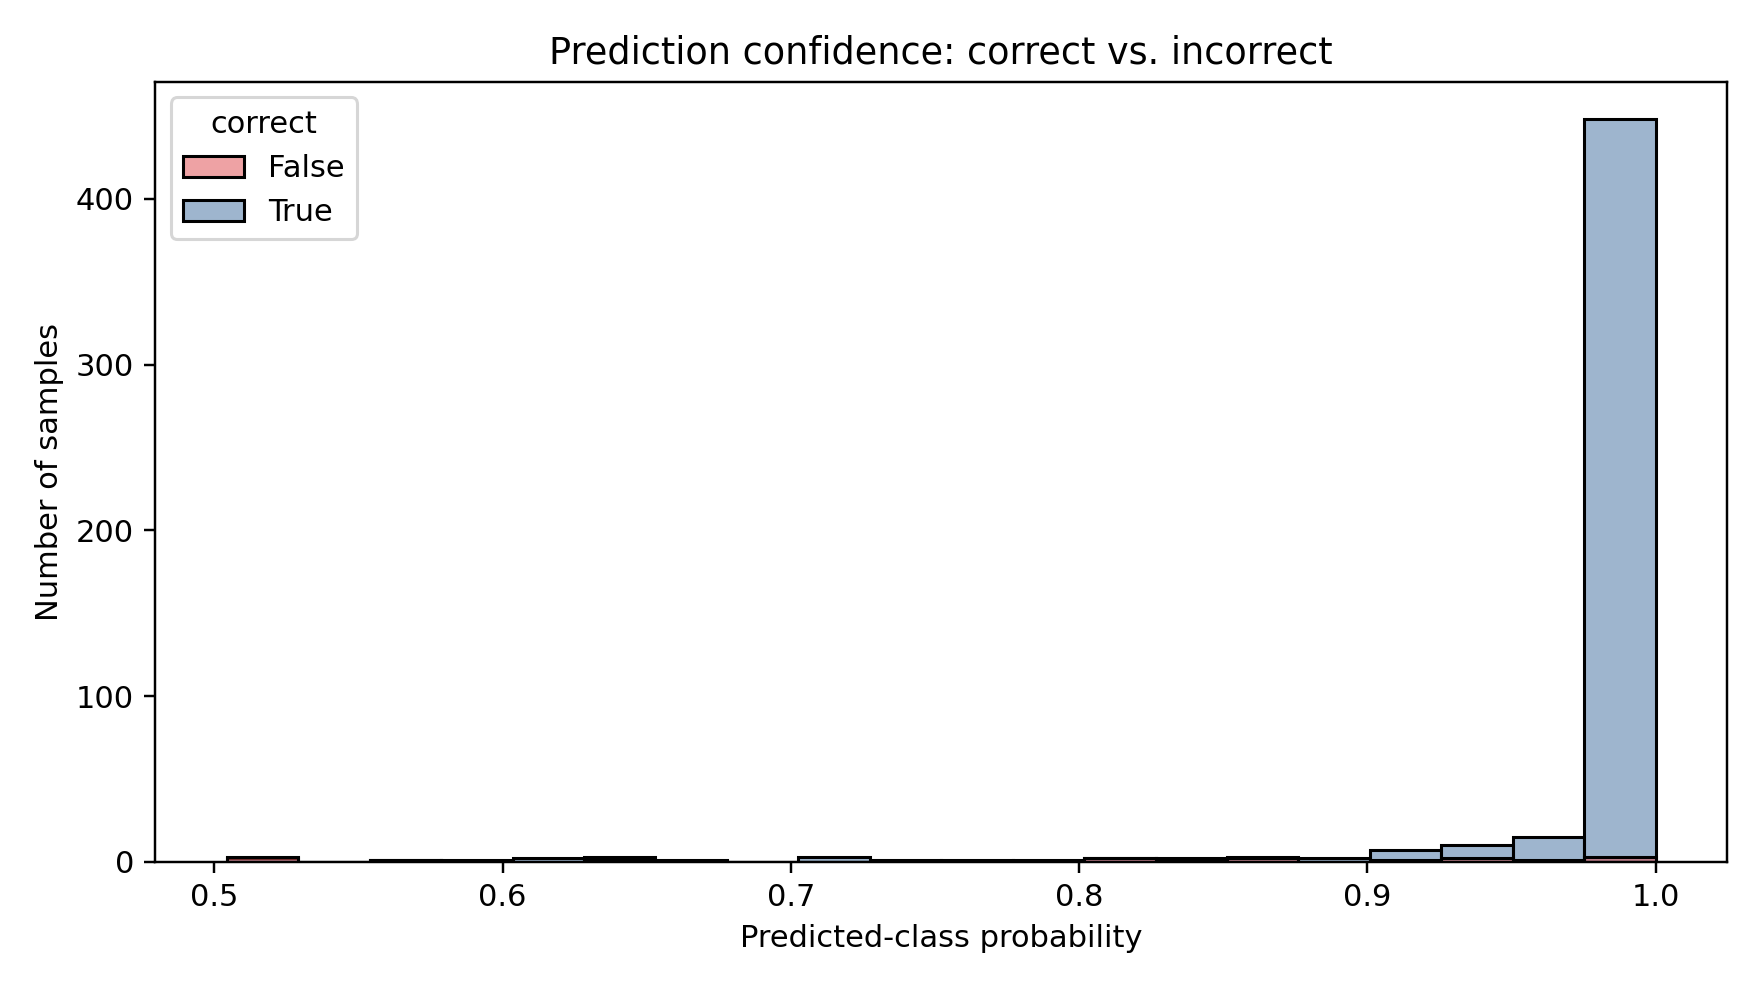
\includegraphics[width=\textwidth,height=0.20\textheight,keepaspectratio]{error_confidence_histogram.png}
\end{column}
\begin{column}{0.48\textwidth}
\begin{block}{Ablation finding}
\begin{itemize}
  \item Frozen head: \(0.8697\) test accuracy.
  \item Layer4 fine-tune: \(0.9406\).
  \item Full fine-tune at \(10^{-4}\): \(0.9617\).
\end{itemize}
\end{block}
\begin{block}{Residual errors}
\begin{itemize}
  \item 20 errors out of 522 test images.
  \item 10 \healthy{}\(\rightarrow\)\unhealthy{} and 10 \unhealthy{}\(\rightarrow\)\healthy{}.
  \item 12 high-confidence errors with confidence \(\ge 0.80\).
\end{itemize}
\end{block}
\end{column}
\end{columns}
\end{frame}

% Slide 9
\begin{frame}{Safety, Ethics, and Takeaways}
\footnotesize
\begin{columns}[T]
\begin{column}{0.48\textwidth}
\begin{block}{Deployment risks}
\begin{itemize}
  \item \healthy{} / \unhealthy{} labels are coarse nutritional proxies.
  \item Food meaning varies by portion size, ingredients, cuisine, and medical context.
  \item A high-accuracy model still makes high-confidence mistakes.
  \item User-uploaded images raise privacy and consent concerns.
\end{itemize}
\end{block}
\end{column}
\begin{column}{0.48\textwidth}
\begin{block}{Conclusion}
\begin{itemize}
  \item Transfer learning is the dominant performance driver.
  \item Best model: \(0.9617\) accuracy and \(0.9944\) ROC AUC.
  \item Current system is suitable as an academic classifier, not an authoritative health tool.
  \item Next steps: calibration, larger backbones, external validation.
\end{itemize}
\end{block}
\end{column}
\end{columns}
\end{frame}

% Slide 10
\normalframetitle
\begin{frame}
\centering
\vspace{0.18\textheight}
{\Huge Thank You}
\end{frame}

\end{document}
